%%%%%%%%%%%%%%%%%%%%%%%%%%%%%%%%%%%%%%%%%%%%%%%%%%%%%%%%%%%%%%%%%%%%%%%%%%%%%
%%%
%%% File: thesis.tex, version 1.9, May 2016
%%%
%%% =============================================
%%% This file contains a template that can be used with the package
%%% cs.sty and LaTeX2e to produce a thesis that meets the requirements
%%% of the Computer Science Department from the Technical University of Cluj-Napoca
%%%%%%%%%%%%%%%%%%%%%%%%%%%%%%%%%%%%%%%%%%%%%%%%%%%%%%%%%%%%%%%%%%%%%%%%%%%%%

\documentclass[12pt,a4paper,twoside]{report}     
\usepackage{cs}              
\usepackage{times}
\usepackage{graphicx}
\usepackage{latexsym}
\usepackage{amsmath,amsbsy}
\usepackage{amssymb}
\usepackage[matrix,arrow]{xy}
\usepackage[T1]{fontenc}
\usepackage{ae,aecompl}
%\usepackage{shortcut} %definitii pentru diacritice; 
\usepackage{amstext}
\usepackage{graphics}
\usepackage[T1]{fontenc}
\usepackage{ae,aecompl}
\usepackage{algorithm}
%\usepackage{algorithmic}
\usepackage{color}
\usepackage{color}
\usepackage{bytefield}
\usepackage{listings} 

\usepackage[hyphens]{url}
\usepackage[hidelinks]{hyperref}
\hypersetup{breaklinks=true}
\urlstyle{same}
\usepackage{cite}



% \mastersthesis
\diplomathesis
% \leftchapter
\centerchapter
% \rightchapter
\singlespace
% \oneandhalfspace
% \doublespace

\renewcommand{\thesisauthor}{Áron KATONA}    %% Your name.
\newcommand{\thesisauthorgroup}{30433}    %% Your group.
\renewcommand{\thesismonth}{}     %% Your month of graduation.
\renewcommand{\thesisyear}{2020}      %% Your year of graduation.
\renewcommand{\thesistitle}{Star Wars inspired scene} 
\renewcommand{\thesissupervisor}{}
\newcommand{\department}{\bf FACULTY OF AUTOMATION AND COMPUTER SCIENCE\\
COMPUTER SCIENCE DEPARTMENT}
\newcommand{\thesis}{}
\newcommand{\utcnlogo}{
\includegraphics[width=15cm]{img/tucn.jpg}}

\newcommand{\uline}[1]{\rule[0pt]{#1}{0.4pt}}
%\renewcommand{\thesisdedication}{P\u{a}rin\c{t}ilor mei}

\begin{document}
%\frontmatter
%\pagestyle{headings}

\newenvironment{definition}[1][Defini\c{t}ie.]{\begin{trivlist}
\item[\hskip \labelsep {\bfseries #1}]}{\end{trivlist}}



%\thesistitle                    %% Generate the title page.
%\authordeclarationpage                %% Generate the declaration page.


\begin{center}
\utcnlogo

\department

\vspace{4cm}

{\bf \thesistitle} %LICENSE THESIS TITLE}

\vspace{1.5cm}


\vspace{6cm}

Name: {\bf \thesisauthor} 

Group: {\bf \thesisauthorgroup}

\vspace{3cm}
{\bf \thesisyear}
\end{center}

\thispagestyle{empty}
\newpage

\pagenumbering{roman}
\setcounter{page}{1}



\tableofcontents
\newpage

\pagenumbering{arabic}
\setcounter{page}{1}
\pagestyle{headings}

 
\chapter{Subject specification} 

The scope of the application is to visualize photo-realistically a scene, which was inspired by the well-known Star Wars saga. The scene presents the desert planet of Tatooine, a key place in the story, where the star wars saga began. The user of the application can explore this planet and meet with some famous characters from the movies.

\subsubsection{Key aspects}

The following aspects were implemented:

\begin{itemize}

\item Camera movement using keyboard and mouse

\begin{itemize}
 \item Preserving the height while moving
\end{itemize}

\item Camera movement animation

\item Translation and rotation in animation

\item Rotation and scaling using keyboard and mouse

\begin{itemize}
 \item Rotation of the sun around an arbitrary axis
\end{itemize}

\item Multiple light sources:

\begin{itemize}
 \item 1 x directional
 \item 2 x point light sources (generic implementation for any number of point lights)
\end{itemize}

\item viewing solid, wireframe objects, polygonal and smooth surfaces

\item texture mapping and materials

\item shadow mapping

\begin{itemize}
 \item Optimization of the light space transformation matrix by adapting to the dimensions to the scene
 
 \item Percentage close filtering
\end{itemize}

\item Animation of object components

\item Collision detection

\item Sandstorm (fog)

\item Skybox for day and for night

\item Handling window resize

\end{itemize}

\chapter{Scenario}

\section{Scene and objects description}

\begin{figure}[ht]
    \centering
    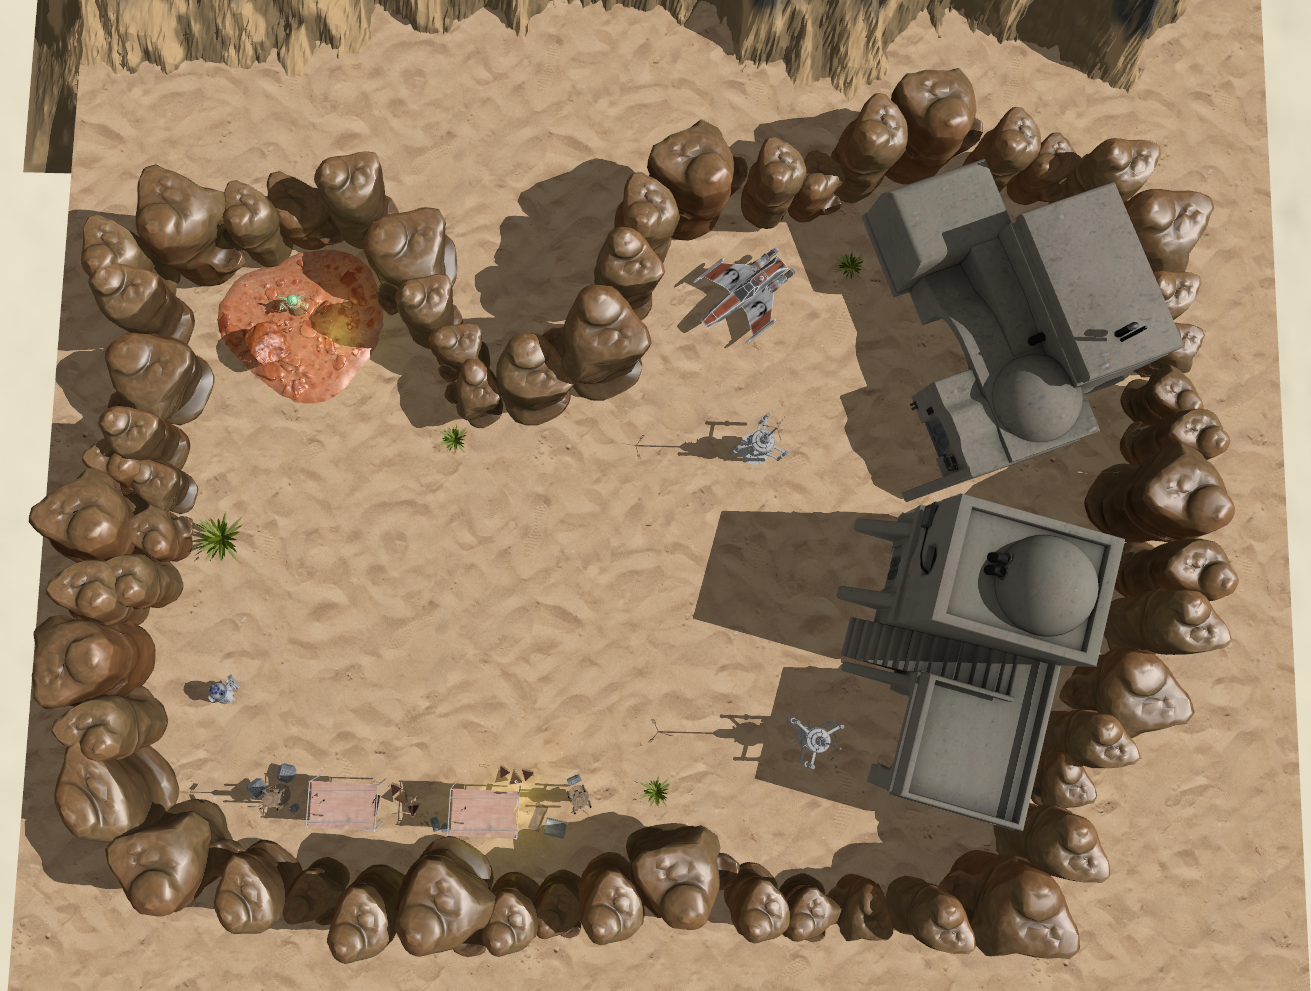
\includegraphics[width=\linewidth]{img/top_view.png}
    \caption{View of the scene from the top}
    \label{fig:top}
\end{figure}

The application uses two \textbf{skyboxes}. For daytime it uses a skybox showing a desert with mountains (Figure \ref{fig:skybox_day}) and for nighttime it uses one which presents a starry sky (Figure \ref{fig:skybox_night}).

The directional light source of the application is the \textbf{sun}, which can be rotated around an \textit{arbitrary axis}. The axis is hard-coded, however it can be changed by modifying a global constant. (Figure \ref{fig:skybox_day}). The skybox also contains a sun at the top. Hovewer it is not a mistake because Tatooine is part of a binary solar system i.e. there are two suns.

Since the scene presents a desert planet, the \textbf{ground} should be covered in sand. This was achieved by mapping a sand texture to a wide, slim rectangular box.

The scene is enclosed by \textbf{boulders}, forming a wall. It serves the purpose of increasing the photorealism by not allowing the user to directly see the skybox. Another important role of them is to block the camera from exiting the scene.

Next to the scene a small \textbf{mountain} is placed which helps building a more realistic view in the distance. In some positions its peak hides the sun, thus projecting a reflection to the scene. (Figure \ref{fig:rock})

In this planet people obtain their daily supply of water by extracting the water molecules form the air. The so cold \textbf{moisture vaporators} have a great importance, thus the scene contains a few of them. (Figure \ref{fig:building})

The scene contains two \textbf{buildings} in the architectural style of the desert worlds. (Figure \ref{fig:building})

In front of the leftmost building, in the corner, one can find a \textbf{Jedi star-ship}. Their symbol is painted on it. When the Jedi knights have individual missions in foreign planets, they usually travel by similar ships, accompanied by only their astromech droid. These droids can repair the ship and can have conversation with their owner. The head of such droid can be seen in behind the pilot cabin. (Figure \ref{fig:ship})

As for any habitable planet, Tatooine has markets in its settlements. A \textbf{fruit stand} was placed in the scene, accompanied by seats, barrels, and other items which can give the viewer the feeling of the marketplaces of the desert planet, like Mos Espa. (Figure \ref{fig:fruit_stand})

A triplet of \textbf{fireflies} are placed above the red fruits, which illuminate the nearby objects with yellow color. The fireflies form a point light source and have the same color as their emitted light. (Figure \ref{fig:fruit_stand})

Next to the fruit stand one can find two comfortable \textbf{seats} with a drink table. These items represent the entertainment of a more elegant class of citizens. (Figure \ref{fig:seats})

\textbf{R2-D2}, the most famous droid in the saga is also present in the scene. He serves an important role in the saga, some consider him a main character. (Figure \ref{fig:r2-d2})

Finally, the most loved creature of the recent years is present in an animation. \textbf{Grogu} aka. \textbf{``Baby Yoda''} is a small 50 year old force sensitive child who became beloved by the fans after its appearance in ``The Mandalorian'' serial. By using the Force, he can do telekinesis and move objects. In this animation we can see him pointing his hand towards the rock, and moving it periodically up-down while also rotating it. (Figure \ref{fig:baby_yoda})

For special effects, a \textbf{fog} was created with sand color to imitate a \textbf{sandstorm} (Figure \ref{fig:fog}).

\begin{figure}
    \centering
    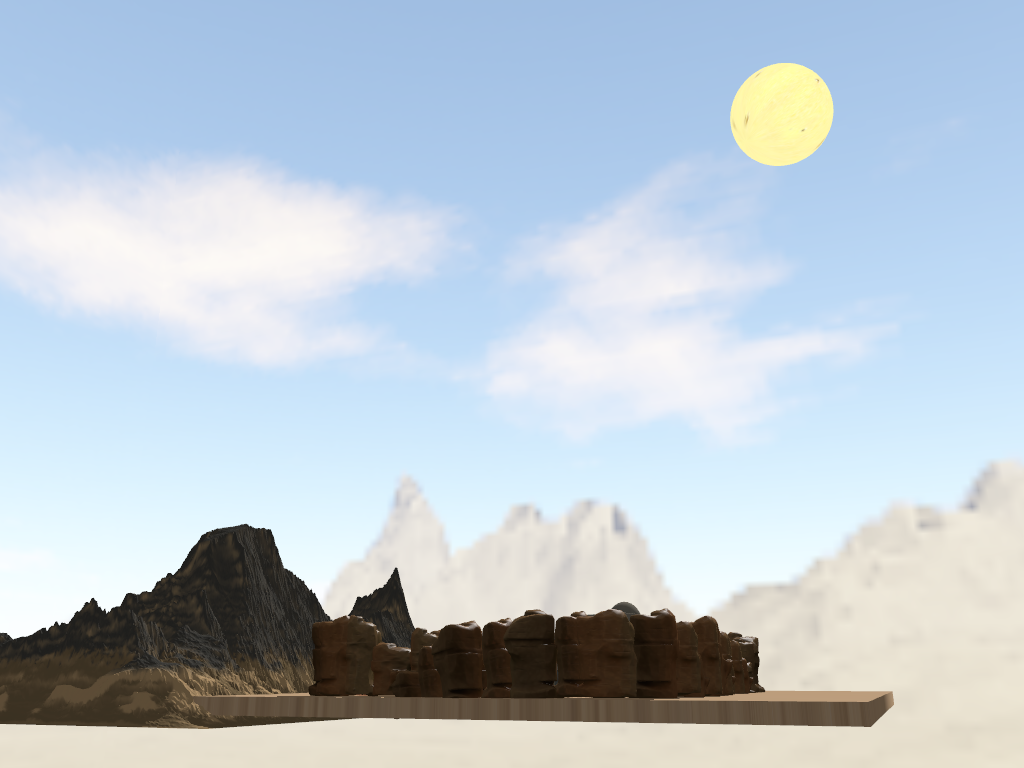
\includegraphics[width=.75\linewidth]{img/skybox_day.png}
    \caption{The scene and the sun enclosed by the daytime skybox}
    \label{fig:skybox_day}
\end{figure}

\begin{figure}
    \centering
    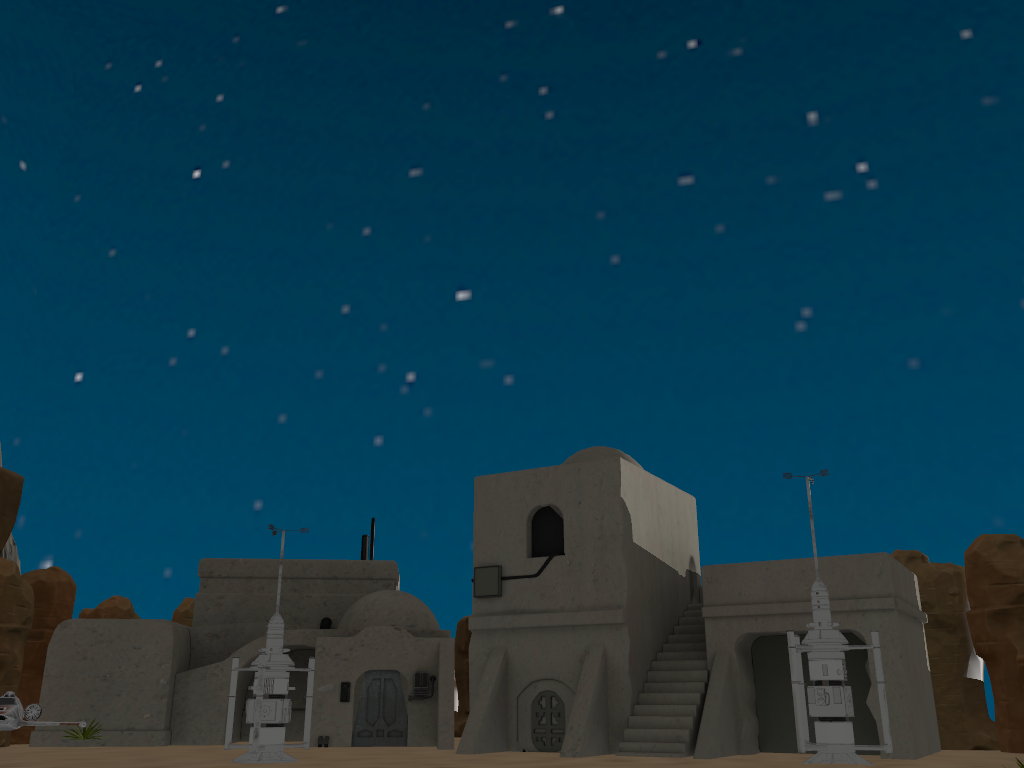
\includegraphics[width=.75\linewidth]{img/skybox_night.png}
    \caption{View of the sky at night}
    \label{fig:skybox_night}
\end{figure}

\begin{figure}
    \centering
    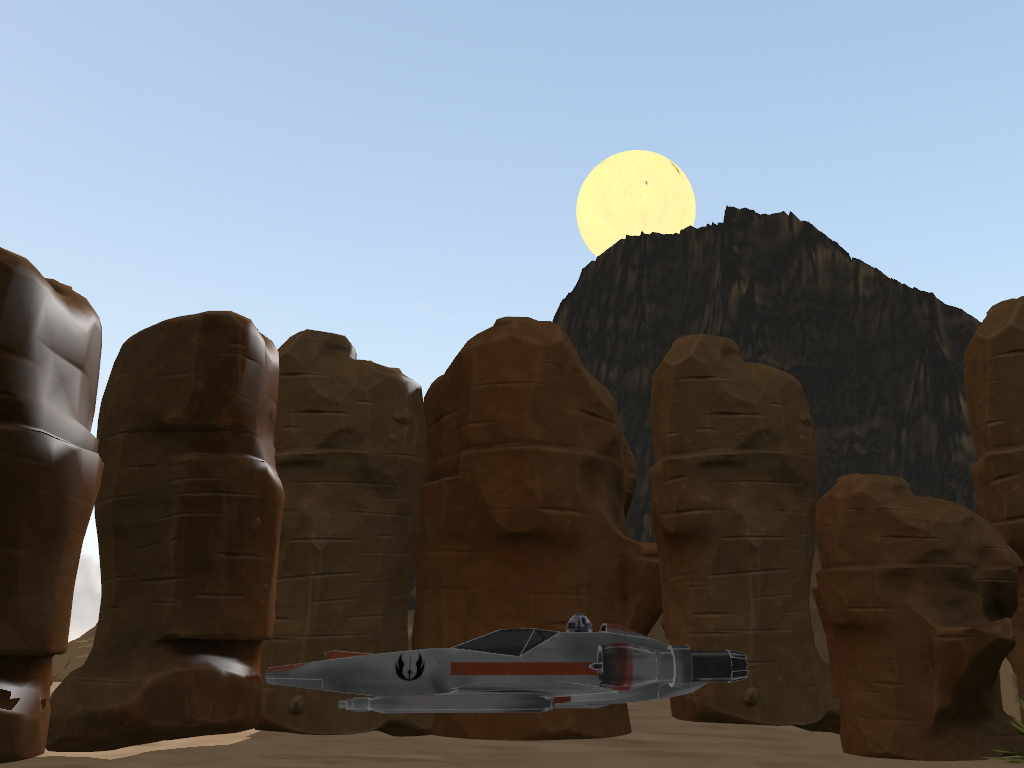
\includegraphics[width=.75\linewidth]{img/rock.png}
    \caption{View of the sun behind the peak of the neighboring mountain}
    \label{fig:rock}
\end{figure}

\begin{figure}
    \centering
    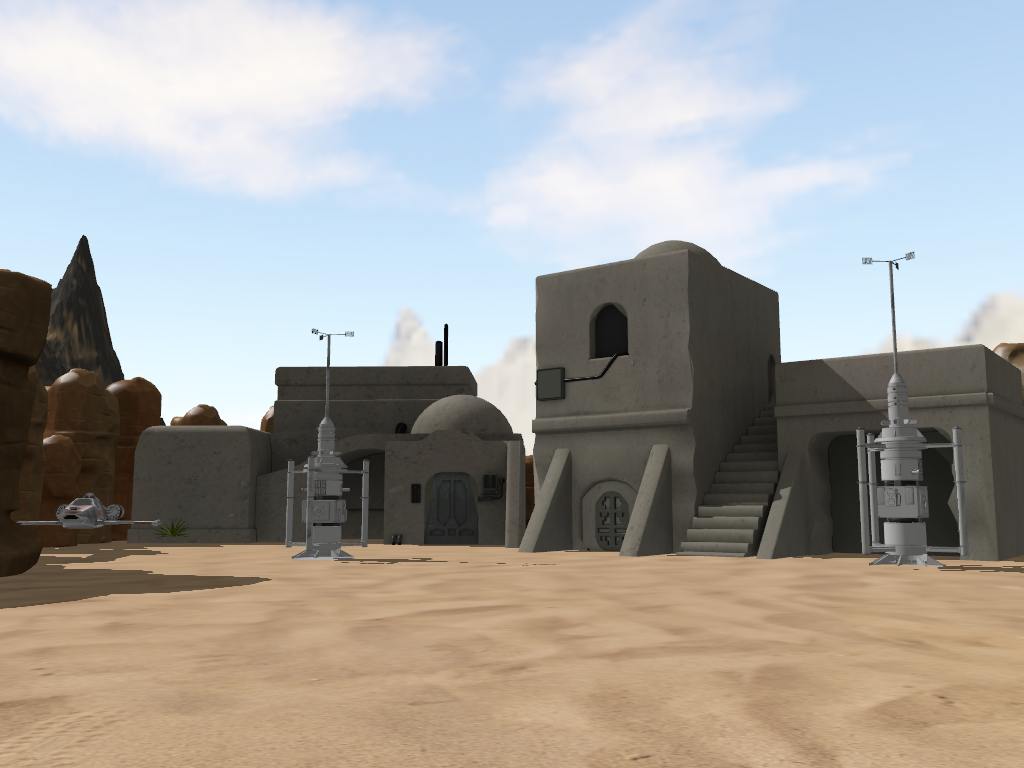
\includegraphics[width=.75\linewidth]{img/building.png}
    \caption{View of the moisture vaporators near the buildings in the morning}
    \label{fig:building}
\end{figure}

\begin{figure}
    \centering
    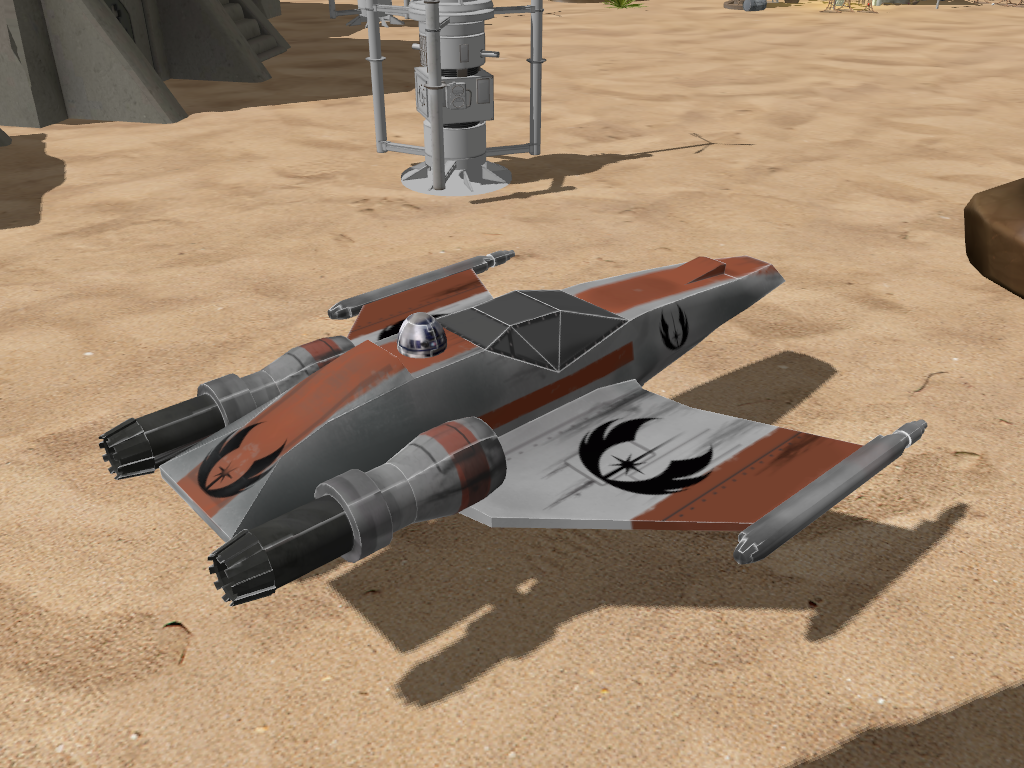
\includegraphics[width=.75\linewidth]{img/ship.png}
    \caption{View of the Jedi ship and its astromech droid}
    \label{fig:ship}
\end{figure}

\begin{figure}
    \centering
    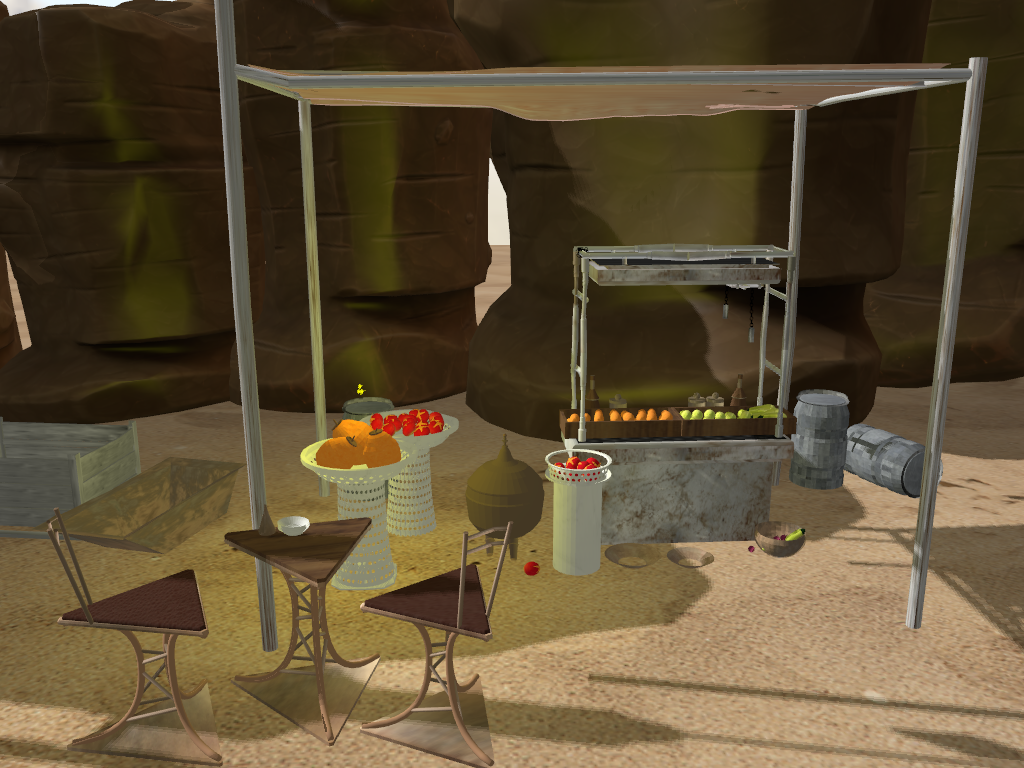
\includegraphics[width=.75\linewidth]{img/fruit_stand.png}
    \caption{View of the fruit stand before sunset, illuminated by the fireflies}
    \label{fig:fruit_stand}
\end{figure}

\begin{figure}
    \centering
    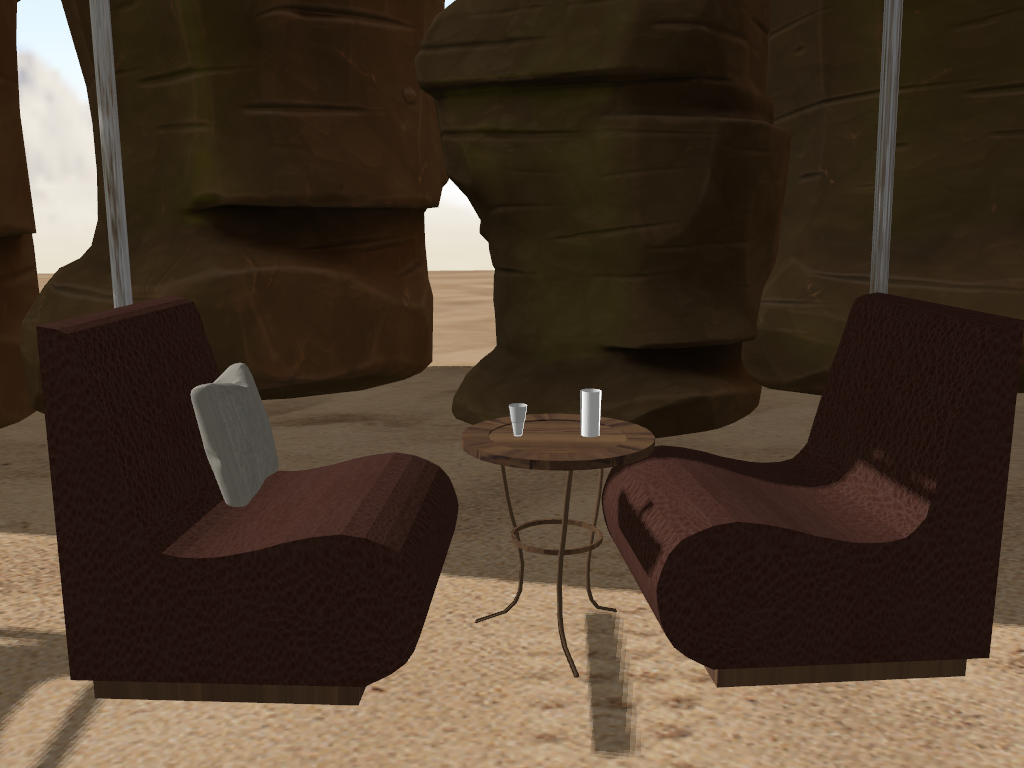
\includegraphics[width=.75\linewidth]{img/seats.png}
    \caption{View of two comfortable seats near a drink table}
    \label{fig:seats}
\end{figure}

\begin{figure}
    \centering
    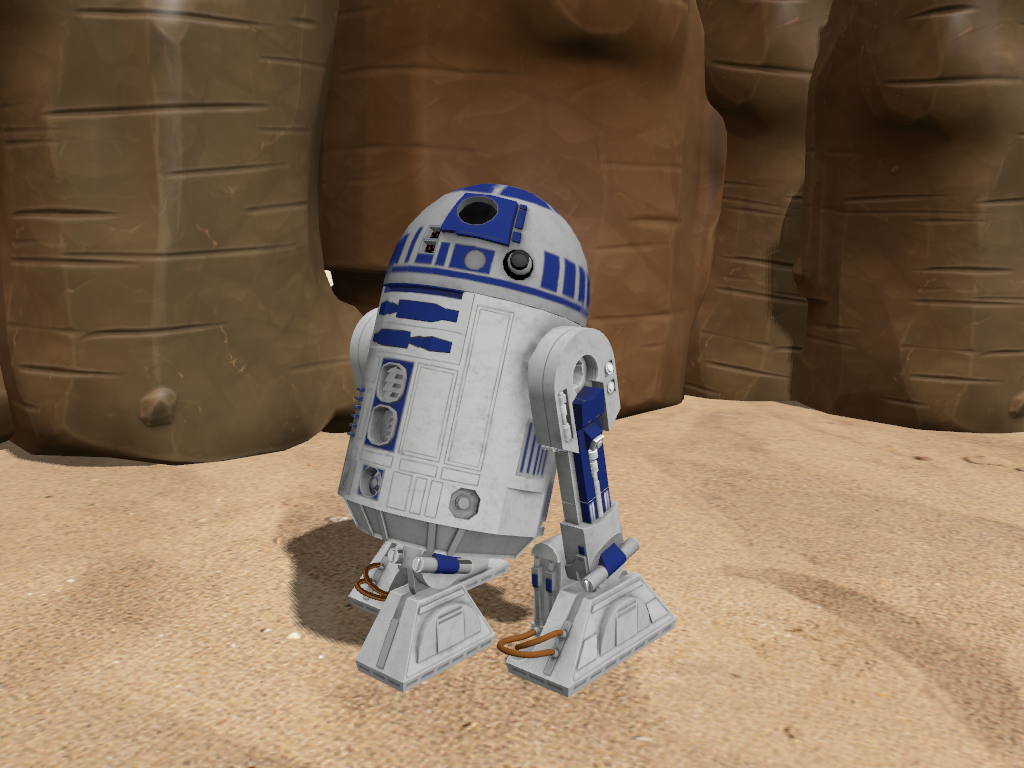
\includegraphics[width=.75\linewidth]{img/r2-d2.png}
    \caption{View of R2-D2 the favorite droid of the fans}
    \label{fig:r2-d2}
\end{figure}

\begin{figure}
    \centering
    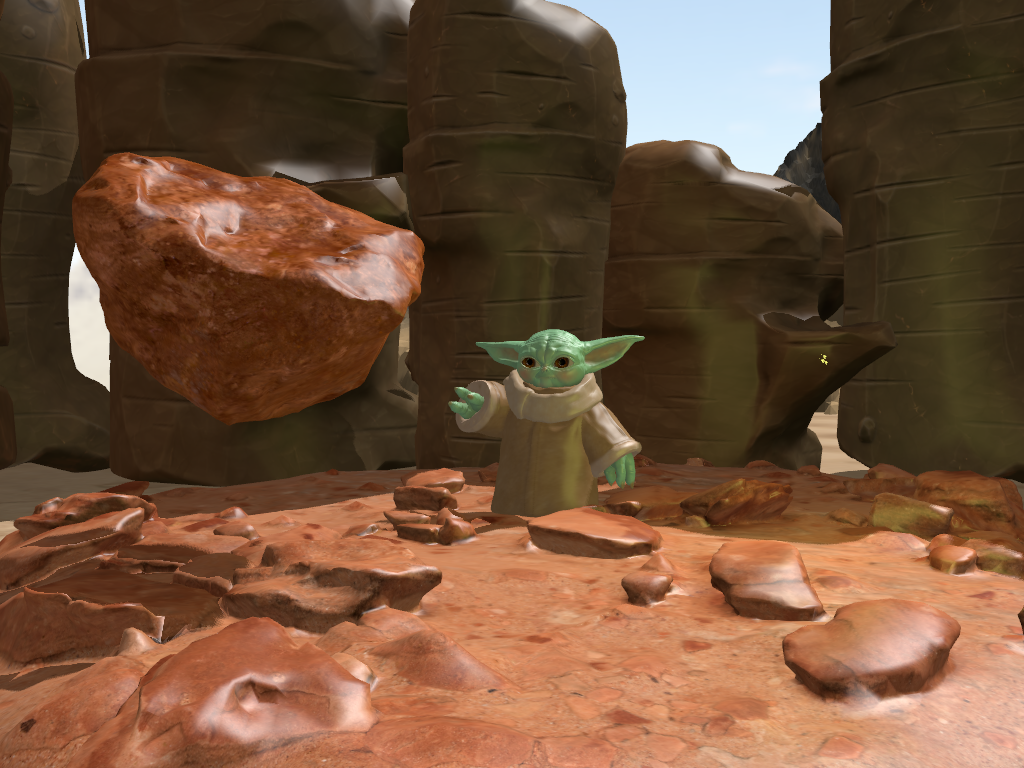
\includegraphics[width=.75\linewidth]{img/baby_yoda.png}
    \caption{View of ``Baby Yoda'' Grogu moving a rock using the force, illuminated by the sun and by fireflies}
    \label{fig:baby_yoda}
\end{figure}

\begin{figure}
    \centering
    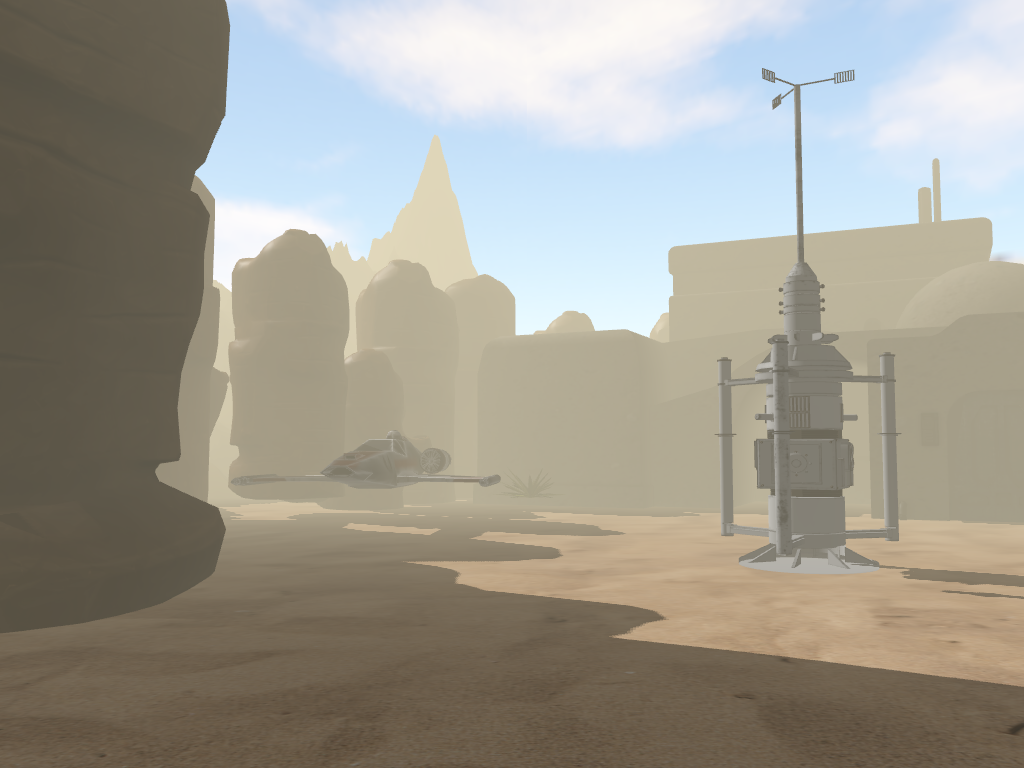
\includegraphics[width=.75\linewidth]{img/fog.png}
    \caption{View of a moisture vaporator in the sandstorm}
    \label{fig:fog}
\end{figure} 

\section{Functionalities} 

A passive functionality is the \textbf{baby yoda animation} (Figure \ref{fig:baby_yoda}), which shows him moving a rock by using the force. The rock is translated and rotated periodically.

The other funtionalities are enumerated in the following list:

\begin{itemize}
 \item \textbf{Rotate the sun} in both directions. If the sun is beyond the horizont, the night scene is showed, otherwise the day scene. This action also changes the light direction.
 
 \item \textbf{Scale the sun}. Only the object is changed. It produces no lighting effect.
 
 \item \textbf{Increase/decrease the fog (sandstorm) density}.
 
 \item \textbf{Move and rotate camera} with keyboard and mouse.
 
 \item \textbf{Activate/deactivate camera animation}. The animation leads the viewer along a predefined path and ignores the keyboard and mouse movement inputs.
 
 \item \textbf{View the depth map} from the point of view of the sun.
 
 \item \textbf{Switch between viewing modes:} wireframe, solid with polygonal surfaces, solid with smooth surfaces 
 
 
\item \textbf{Activate/deactivate collision detection} 
\end{itemize}




\chapter{Implementation details}

\section{Functions and algorithms} 

\subsection{Lighting}

The application implements the \textbf{Blinn-Phong} lighting model in the \verb|basic.frag| shader. The algorithm is the same as in the laboratory works, but the code is modified to tailor it to the application:

\begin{itemize}
 \item The fields of the directional and point lights are sent in structures.
 \item The ambient, diffuse and specular coefficients are constructed in separate variables, and summed together at the end.
 \item \textit{Multiple point lights} can be sent from the application to the shader, and each will be considered in the final color.
 \item Other refactoring to increase code reuse.
\end{itemize}

For the lighting of the \textbf{sun} it was needed only to apply its diffuse texture without any modifiers. The \textbf{fireflies} however are colored to the color of their emitted light. Thus for them another shader was created which draws these objects with a single color.






\subsection{Shadows}

The application applies the \textbf{shadow mapping} algorithm from the laboratory guide, however it is \textit{improved} to provide higher quality results. The shadows are only considered for the directional light source.

\subsubsection{Percentage-close filtering}

\verb|basic.frag|

In order to provide softer shadows the percentage-close filtering technique \cite{learnopengl} was used. When a fragment's depth is compared to the corresponding value in the depth map, the depth is compared also with the 8 neighbors of the mapped pixel in the texture. At the end the average of the shadow values will be the final shadow value of the fragment.

\subsubsection{Light space transformation matrix optimization}

\verb|shadow.cpp|

The goal is to create a correct view transformation and to set the bounds of the orthographic projection such that the viewing volume contains all the scene and its size is minimal.

The direction of the light is the same as the direction of the sun. It is normalized, therefore by adding $(0,0,0)$ to it, it can be considered as a point from unit distance from the origin towards the light direction. This point $P_c(x, y, z)$ is the \textbf{camera position} for the view matrix.

The \textbf{up vector} is computed differently. The camera looks at the origin, but it's height is not always 0. Therefore the up vector should not be always the OY axis. In the computation I considered two cases. In the \textbf{first case}, the camera is in the XOZ plane, i.e. $y = 0$. In this case the up vector is $(0, 1, 0)$. In \textbf{the second case} the camera is above the scene, i.e. $y > 0$. In this case the up vector is the vector which is perpendicular to the viewing direction and passes through $P_c = (x, y, z)$ and another point on the OY $P = (0, y', 0)$. After some trigonometric calculations I obtained the following formula:

\begin{equation}
 y' - y = \frac{x^2 + z^2}{y},\; y > 0
\end{equation}

Thus the up vector in the second case is:

\begin{equation}
\label{eq:up_up}
U       = P - P_c 
        = (0, y', 0) - (x, y, z) 
        = \langle-x, y - y', -z\rangle
        = \langle-x, \frac{x^2 + z^2}{y}, -z\rangle
,\; y > 0
\end{equation}

In the \textbf{third case}, the camera is below the scene, thus $y < 0$. If we apply formula \ref{eq:up_up} the camera will look at the scene upside down. Therefore in this case the up vector is negated.

\begin{equation}
\label{eq:up_down}
U       = P_c - P
        = \langle x, \frac{x^2 + z^2}{-y}, z\rangle
,\; y < 0
\end{equation}

After the view matrix is obtained, the next step is to calculate the orthographic \textbf{projection matrix}. An option could be to set view volume bounds to the largest absolute value from the scene coordinates. However this would consider also some unneeded regions, thus lowering the final quality.

To \textbf{calculate the view volume bounds}, the \textit{bounding box} of the scene was computed which holds the maximum and minimum $x$, $y$ and $z$ values of the vertices of the scene. These 8 coordinates (vertices of the bounding box) are then \textbf{transformed to the light space}. After that the $z$ values are reversed. Then we find the maximum and minimum coordinates from these eight. The resulting six coordinates ($x_{min}, x_{max}, y_{min}, y_{max}, z_{min}, z_{max}$) will be the bounds of the viewing volume in the orthographic projection. \textbf{The resulting viewing volume contains entirely the scene, and its size is minimal.}






\subsection{Sun rotation}

\verb|Sun.cpp|, \verb|util.cpp|

The goal is to \textbf{rotate the sun around an arbitrary axis}, which passes through the origin, with a given angle and radius.

The first step is to normalize the given axis. Then we need to find a vector which is perpendicular to the axis. There are infinite number of such vectors so any of them can be chosen. Therefore the perpendicular vector is obtained by a cross product between the axis and another non-parallel vector: for $\langle 1, 0, 0 \rangle$ we choose $\langle 0, 1, 0 \rangle$, and for any other vector we choose $\langle 1, 0, 0 \rangle$.

After the perpendicular vector is obtained, the sun, whose initial position is at the origin, is \textbf{translated} towards this direction a number of units that is equal to the radius. After transformation the distance between the sun and the given axis in exactly the radius.

To \textbf{rotate the sun }with a given angle, a rotation matrix must be created which rotates it around the given axis. If we apply this transformation after the previous translation, the \textbf{radius is preserved} thus the goal is achieved.







\subsection{Camera animation}

\verb|CameraAnimation.cpp|

To animate the camera, \textbf{centripetal Catmull-Rom splines} \cite{splineCatmullRom} are created. The algorithm interpolates the points between two control points $P_1$, $P_2$ when another two points are given: $P_0$, $P_3$. I adapted the algorithm in order to animate the camera. 

A list of \textbf{control points} are defined which describe the route of the camera. The points are placed around the objects that should be highlighted.

To \textbf{store the animation state}, the index of the current point is saved in a field, the current point being the one the camera just surpassed. Another variable is stored, $t$, which is the parameter in the curve between the current point and the next point. This defines the next interpolated point.

To not depend on the framerate, the duration between each animation is measured and added to $t$ after being multiplied by the animation speed. This way at each animation step the next point is calculated.

Before calling the algorithm one must \textbf{select four control points}, which will be the current control point, the previous one in the list, and the next two.

The point obtained by the algorithm for the given $t$ will be the new \textbf{camera position}. The \textbf{camera target} is obtained by computing the direction from the previous camera position to the current one and adding it to the current camera position. This way the \textbf{camera always looks at the direction of its movement}, it follows the spline.

After the \textbf{camera reaches the next control point}, the two progress variables are updated: $t$ set to 0, and the current control point variable refers to the next one.





\subsection{Camera movement in plane}

The goal is the preserve the height of the camera and move it only in the XOZ plane. 

To implement it, the $y$ coordinates in the camera front direction and in the camera right direction are ignored. The resulting vectors are normalized and used for calculating the next camera position.





\subsection{Sandstorm (fog) computation}

The algorithm is the same as in the laboratory guide. Only the color is changed to resemble to a sandstorm.





\subsection{Polygonal surface visualization}

\verb|basic.geom|

To draw polygonal surfaces, the surface normal of each triangle must be computed and sent to the fragment shader. This is done in the geometry shader. The cross product is calculated between two edges of the triangle. Then the resulting vector is multiplied with the normal matrix and normalized \cite{learnopengl}.





\subsection{Collision detection}

To detect collisions, the application compares the bounding boxes of the objects. 

In the \verb|Model3D| class, while loading the object from a file, the class saves the minimum and maximum coordinates for each mesh in a list. After that, from these bounding boxes it computes the overall \textbf{object bounding box};

The \verb|Model| class which stores its own model matrix, must override the \verb|getBoundingBox()| and \verb|getMeshBoundingBoxes()| methods, because it must apply the modeling transformation to those coordinates.

The \verb|Model3D| class defines the \verb|collidesWith()| function which verifies whether a given bounding box collides with the model or not. To do this it first \textbf{compares with the object bounding box}, than only if they collide, \textbf{compares it to the mesh bounding boxes}.

The main application stores in a list the pointers to the models for which collision detection must be executed. When the user tries to move the camera, the camera bounding box is  
sent to the \verb|collidesWith()| method of each model in this list. In case of a collision the camera is not moved.





\subsection{Animation of object components}

\verb|BabyYoda.cpp|

``Baby Yoda'' moves the rock using the force. To achieve this animation the rock must be separately transformed than the other parts of the object. The rock, the ground and the creature are a single object, loaded using the \verb|Model3D| class.

To achieve the transformation of a single mesh, the \verb|Draw()| function is overridden. In this function before drawing the mesh of the rock, a new model matrix is sent to the shader. After the mesh is drawn, the model matrix is changed back to the one stored inside the \verb|Model| superclass.

\section{Graphics model}

The objects are represented in polygonal form, read from ``.obj'' files. Textures are applied on them based on the material files: ``.mtl''.

\section{Data structures} 

The \verb|BoundingBox| data structure holds the minimum and maximum values of an object in two vectors: one for the lowest coordinates, one for the highest coordinates.

Additional data structures were created for storing the data which will be sent to the shaders. These are the same as the ones defined in the shaders. The enclosing modules implement methods for transmitting the structure to the shader. These types of data structures are:

\begin{enumerate}
 \item DirLight
 \item PointLight
 \item Fog
\end{enumerate}

\section{Class hierarchy} 


To improve the performance, one design goal was to compute or transmit data only when needed. Therefore the camera, projection, light space transformation matrices, the fog density, the light direction and all other variable uniform values are sent to the shaders only when they change. The constant uniform values are sent only at the beginning of the program. In order to update the shaders when a uniform value changes, pointers to shaders are stored in lists, for each set of uniform variables a separate list was created. On the change of a value, the corresponding list is traversed and each shader is updated with the new value.

As for the model and normal matrices, they must be sent to the shader each time they are drawn. However the calculation of these matrices can be omitted if no other transformation was applied to the model. For this purpose, the \verb|Model| class was created which extends from the \verb|Model3D| class. It stores the model and normal matrices, which can be requested from it before the \verb|Draw()| method is called.

The \verb|ColoredModel| class extend from the \verb|Model| class, by also storing a \verb|color| field.

The \verb|BabyYoda| class extend from the \verb|Model| class, by providing \verb|startAnimation()| and \verb|stopAnimation()| methods and overriding the \verb|Draw()| function to draw the mesh of the rock using a different model matrix.

The \verb|Sun| class extend from the \verb|Model3D| class. Instead of storing a single model matrix, it stores separately the rotation, translation and scale matrices. Therefore in the future it can perform additional rotations and scalings. This class performs rotation around a given axis with a given radius and angle.


\chapter{User manual}

\paragraph{Key Bindings}

\begin{center}
 \begin{tabular}{| c | l |} 
 \hline
 Key & Action \\ [0.5ex] 
 \hline\hline
 W & Move camera forward\\ 
 \hline
 A & Move camera left\\ 
 \hline
 S & Move camera backward\\ 
 \hline
 D & Move camera right\\ 
 \hline
 Mouse right & Rotate camera to right \\ 
 \hline
 Mouse left & Rotate camera to left \\ 
 \hline
 Mouse up & Rotate camera upwards \\ 
 \hline
 Mouse down & Rotate camera downwards \\ 
 \hline
 E & Rotate sun clockwise \\
 \hline
 Q & Rotate sun counterclockwise \\
 \hline
 CTRL + E & Scale up the sun \\
 \hline
 CTRL + Q & Scale down the sun \\
 \hline
 LSHIFT + E & Increase fog density \\
 \hline
 LSHIFT + Q & Decrease fog density \\
 \hline
 M & Show/Hide depth map \\
 \hline
 V & Toggle between view modes: solid + smooth, solid + polygonal, wireframe  \\
 \hline
 C & Start/Stop camera animation \\
 \hline
 B & Enable/Disable collision detection \\ [1ex] 
 \hline
\end{tabular}
\end{center}


\chapter{Conclusions and further developments}

This application was a great opportunity to put together the concepts learned at the laboratories. Moreover it provided challenges which required mathematical and programming skills.

\textbf{The application can be further developed by:}

\begin{itemize}
 \item Adding spotlights and more point lights
 \item Animating R2-D2
 \item Creating logic for controlling the ship, including the collision detection
 \item Extending the scene with more detailed models
\end{itemize}



\Urlmuskip=0mu plus 1mu
%\addcontentsline {toc}{chapter}{Bibliography} 
\bibliographystyle{IEEEtran} 
\bibliography{documentation}%same file name as for .bib

\end{document}
